\documentclass[12pt,openright,a4paper]{article}

\usepackage{hyperref}
\usepackage[T1]{fontenc}
\usepackage[utf8]{inputenc}
\usepackage[italian]{babel}
\usepackage{amsmath}
\usepackage{amssymb}
\usepackage{caption}
\usepackage{graphicx, floatflt}
\usepackage{booktabs}
\usepackage{textcomp}
\usepackage{subfig}

% permette di inserire le note a margine
\usepackage{marginnote}


\begin{document}
\title{Caratterizzazione e Clustering di Matrici di Correlazione ADNI-2 Tramite Distribuzione di Wishart}
\author{Carlo Mengucci}

\maketitle

\tableofcontents

\section{Introduzione}

In questo estratto vengono presentati i risultati di \textit{clustering} e \textit{classificazione} per soggetti ADNI-2, di cui sono state analizzate le matrici di correlazione ottenute tramite elaborazione in Macrovoxel, utilizzando la \textit{Distribuzione di Wishart} come ipotesi nulla.

Vengono inoltre presentati sinteticamente l'algoritmo e la \textit{pipeline} di \textit{cross-validazione} utilizzati.

\section{Struttura e Utilizzo del Database}

Dei 403 soggetti totali sono stati utilizzati 232 soggetti a seguito di operazioni di filtraggio e dell'individuazione di discrepanze nelle procedure di normalizzazione. E' infatti possibile riscontrare la presenza di due gruppi distinti all'interno del database, dei quali è stato preso in considerazione il più numeroso.

I 232 soggetti utilizzati per l'elaborazione finale sono stati divisi per il \textit{training} utilizzando la sola discriminante della conversione. Sono pertanto utilizzate le labels \textit{NC (Non-Converters)}  e \textit{AD (Alzheimer Diagnosis)} per il clustering; la presenza di soggetti per il gruppo \textit{AD} è del $63 \% $ mentre il restante  $37 \%$ dei 232 soggetti considerati appartiene al gruppo \textit{NC}.

Ad ogni soggetto è associata una matrice di correlazione $N\times N$, $N=549$, Ognuno degli N elementi rappresenta un \textit{Macrovoxel} di cui è estratta la correlazione \textit{topologica} rispetto a tutte le altre componenti del sistema. Ogni \textit{Macrovoxel} è definito su un insieme di $3\cdot10^3$ Voxel.

\section{Distribuzione di Wishart e Definizione delle Condizioni di Applicazione }

\subsection{Definizione della Distribuzione di Wishart}

La distribuzione di Wishart consiste in una famiglia di distribuzioni per \textit{matrici simmetriche definite positive}.

\textit{Def.} Siano $X_1...X_n$ indipendenti $N_p(0,\Sigma)$ distribuiti, tali da formare una matrice di dati $p\times n$, $X=[X_1...X_n]$.
La distribuzione di \textit{matrici random} $p\times p$, $M=XX'=\Sigma^n_{i=1}X_iX_i'$ è una distribuzione di Wishart. \cite{AMS}

La matrice random $M_{p\times p}=\Sigma^n_{i=1}X_iX_i'$ segue una distribuzione di Wishart a $n$ gradi di libertà e \textit{matrice di covarianza} $\Sigma$ ed è definita $M\sim W_p(n, \Sigma)$.
Per $n\geq p$ la \textit{pdf} di $M$ assume la forma   \footnote{\textit{Nota: $\|\Sigma , N \| = det (\Sigma , M)$}}:  
\begin{equation}
f(M)=\frac{1}{2^{\frac{np}{2}}\Gamma_p(\frac{n}{2})\|\Sigma\|^{\frac{n}{2}}}\|M\|^{\frac{n-p-1}{2}}exp[-\frac{1}{2}trace(\Sigma^{-1}M)]
\label{Wishat-pdf}
\end{equation}

La Wishart può essere interpretata come l'estensione multivariata di una distribuzione $\chi^2$.



\subsection{Definizione delle Condizioni di Applicazione}

Le matrici di correlazione sono per definizione simmetriche definite positive.

Il numero $n$ di gradi di libertà del sistema è dato dal campionamento $(n=3\cdot 10^3)$ del singolo Macrovoxel.

Utilizzando come matrice di scala la matrice data dalla media delle matrici di correlazione delle due categorie di soggetti, è possibile stimare la Wishart attesa per le categorie stesse.

Un approccio di questo tipo permetterebbe la classificazione ogni soggetto in base alla propria distanza dalle distribuzioni rappresentative delle categorie, in termini di \textit{LogPDF}, come definito dalla eq.(\ref{pdf-score}):

\begin{equation}
score_{subj }= logP_{W}(\Sigma_{subj}\mid n, \hat{\Sigma}_{AD})-logP_{W}(\Sigma_{subj}\mid n,\hat{\Sigma}_{NC})
\label{pdf-score}
\end{equation}

dove $\Sigma_{subj}$ rappresenta la matrice del singolo soggetto e $\hat{\Sigma}_{AD,NC}$ è la matrice media di categoria.

L'algoritmo implementato rende possibile la stima dello score, relativo alla distanza dalle distribuzioni attese per le categorie, \textit{feature} per \textit{feature}. Per ogni paziente viene infatti calcolato lo \textit{score} definito dall' eq.~(\ref{pdf-score}) eliminando di iterazione in iterazione una diversa componente del sistema; in questo modo è possibile stimare il peso che ogni \textit{feature} possiede all'interno del sistema stesso.

Nel caso presente le \textit{features} sono le componenti  della matrice di correlazione associata al soggetto, ossia i 549 \textit{Macrovoxel} rappresentativi del sistema.

\section{Pipeline}

\begin{figure}[!h]
\centering
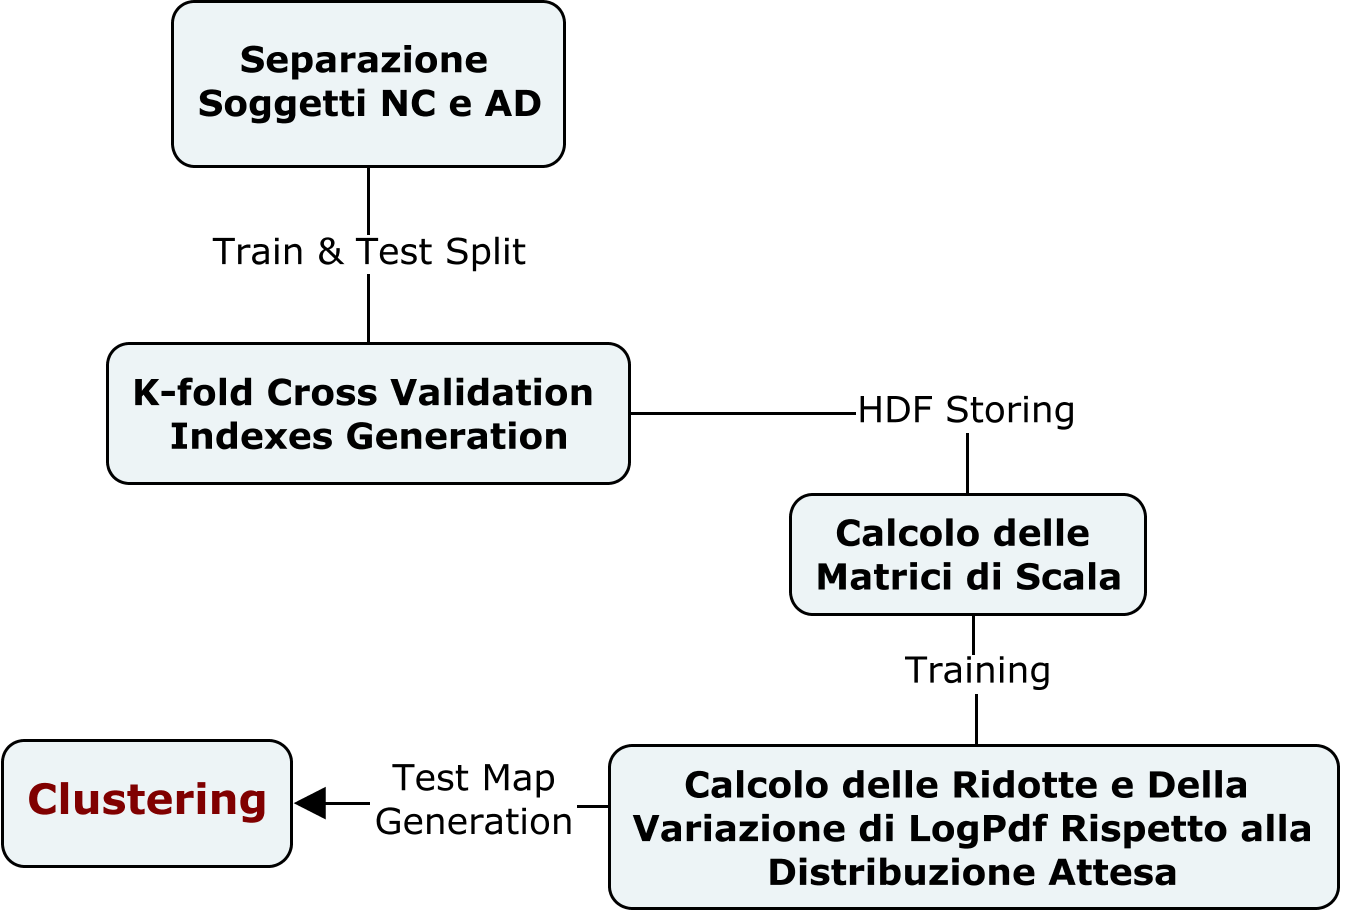
\includegraphics[scale=0.18]{ADNI-alg}
\caption{\textit{Schema di Workflow della pipeline di elaborazione}}
\label{ADNI-alg}
\end{figure}

In figura (\ref{ADNI-alg}) è riportato lo schema di funzionamento dell'intera pipeline. Viene testata la capacità di discriminare tra \textit{NC} e \textit{AD} attraverso un processo di \textit{supervised learning}.

A seguito di una divisione iniziale nelle due classi, vengono separati i soggetti in \textit{train} e \textit{test} secondo il classico split $90 \%- 10 \%$ per ogni batch della \textit{K-fold cross-validation}.

Da ogni batch di training è calcolata la matrice di scala da cui è generata la distribuzione che viene confrontata con il corrispettivo batch di test.

Per ogni soggetto dei batch di test è infine generato un vettore contenente gli \textit{scores} relativi alle singole features, i quali vanno a comporre le mappe finali su cui vengono effettuati clustering e classificazione.

Per il clustering è stata utilizzata una metrica di tipo \textit{City Block} mentre la separazione è stata effettuata utilizzando una SVM a \textit{Kernel Lineare} e parametro $C=1$. Gli score di classificazione sono quindi stimati tramite una cross-validazione 10-fold stratificata.

\section{Risultati}

Come riportato in figura (\ref{logpdf-clustering10}), l'utilizzo degli scores relativi alle singole features permette non solo una buona separazione fra i gruppi NC e AD, ma fornisce anche informazioni su quali siano i gruppi di features più determinanti nella classificazione dei soggetti.

In figura (\ref{logpdf-dist}) sono invece riportate le distribuzioni relative alla somma degli scores dei singoli pazienti. L'informazione viene cioè ridotta ad un singolo score per paziente; ciò non inficia tuttavia la capacità di discriminazione rappresentata dalla forte distinzione tra i due picchi.

Questo risultato è confermato anche dalla performance della SVM che fornisce un'\textit{accuracy} di classificazione del $100\%$.

\begin{figure}[!h]
\centering
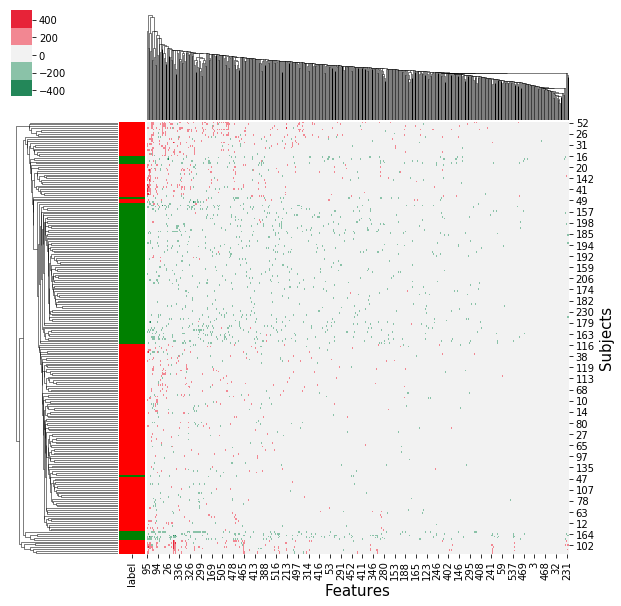
\includegraphics[scale=0.5]{logpdf-clustering10}
\caption{\textit{Risultato del Clustering. Il gradiente di colore è relativo alla significatività delle Features nel stabilire l'appartenenza all'una o all'altra categoria. In verde sono rappresentati i soggetti NC ed in rosso i soggetti AD. }}
\label{logpdf-clustering10}
\end{figure}

\begin{figure}[!h]
\centering
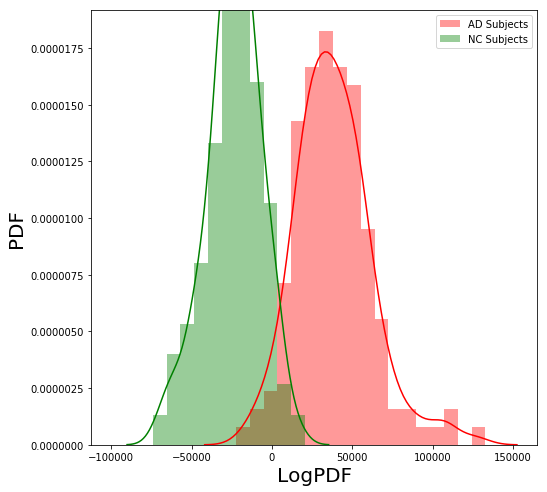
\includegraphics[scale=0.6]{logpdf-dist}
\caption{\textit{Distribuzioni della somma degli scores per paziente. Le classi sono ben distinte anche riducendo ad un unico score l'informazione sui soggetti.}}
\label{logpdf-dist}
\end{figure}


\clearpage

\begin{thebibliography}{99}

\bibitem {AMS}
Hardle, Wolfgang and Leopold Simar

\emph{Applied Multivariate Statistical Analysis}

Heidelberg: Springer Berlin Heidelberg, 2012

\end{thebibliography}

\end{document}